\input{../../input/main}

\begin{document}

\begin{center}
  \Large{\textbf{Городской центр физического образования, 10 класс.}\\
  \textit{Серия 24, 23 апреля 2015.}}
\end{center}

\begin{center}
  \Large\textbf{ Кое-что о циркуляции. }
\end{center}

\task{ Найдите распределение индукции магнитного поля вокруг
  бесконечного прямого провода, по которому течет ток $I$. }

\task{ Какое распределение токов может создавать однородное магнитное
  поле? }

\taskpic{ Как показали эксперименты Ж.-Б. Био и Ф. Савара 1820 года,
  магнитное поле длинного провода с током убывает обратно
  пропорционально расстоянию от длинного прямого провода. Четыре очень
  длинных прямых провода с протекающими по ним равными по модулю
  постоянными токами расположены параллельно друг другу так, как
  показано на рисунке (сечения проводов плоскостью рисунка находятся в
  вершинах квадрата). Известно, что модуль вектора индукции магнитного
  поля, создаваемого одним проводом в соседней с ним вершине этого
  квадрата, равен $B$, а поле самого провода на его оси равно
  нулю. Найдите модуль суммарного вектора магнитной индукции в каждой
  вершине указанного квадрата. Найдите также модуль вектора индукции
  магнитного поля в центре этого квадрата. }
{
  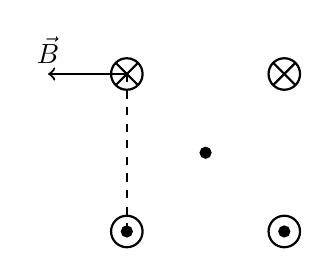
\begin{tikzpicture}
    \draw[thick] (0,0) circle (0.2cm);
    \draw[thick] (0,0) -- ++(45:0.2cm) -- ++(225:0.4cm);
    \draw[thick] (0,0) -- ++(135:0.2cm) -- ++(315:0.4cm);
    \draw[thick] (2,0) circle (0.2cm);
    \draw[thick] (2,0) -- ++(45:0.2cm) -- ++(225:0.4cm);
    \draw[thick] (2,0) -- ++(135:0.2cm) -- ++(315:0.4cm);
    \draw[thick] (0,-2) circle (0.2cm);
    \draw[fill=black] (0,-2) circle (0.07cm);
    \draw[thick] (2,-2) circle (0.2cm);
    \draw[fill=black] (2,-2) circle (0.07cm);
    \draw[fill=black] (1,-1) circle (0.07cm);
    \draw[dashed,thick] (0,-2) -- (0,0);
    \draw[thick,->] (0,0) -- ++(left:1cm) node[above] {$\vec{B}$}; 
  \end{tikzpicture}
}

\task{ Жёсткий металлический изолированный провод изогнут в форме
  пятиконечной звезды; по нему идет электрический ток $I$. Провод
  лежит на столе в магнитном поле как изображено на рисунке. Магнитное
  поле индукции $B$ перпендикулярно поверхности стола, слева от линии
  $AA'$ оно направлено вниз, а справа --- вверх. Длина одной стороны
  клеточки на рисунке равна $d$. Определить силу, действующую со
  стороны поля на провод. }
\begin{center}
  \begin{tikzpicture}
    \draw[step=0.5cm] (-3,-3) grid (3,3);
    \draw[ultra thick,marrow] (-3,-2) -- (1.5,2.5) -- (1.5,-2.5) -- (-3,2) --
    (3,0) -- (-3,-2);
    \draw[line width=0.15cm] (0,3) node[above] {$A$} -- (0,-3)
    node[below] {$A'$};
    \draw[very thick] (4,0) circle (0.2cm);
    \draw[fill=black] (4,0) circle (0.07cm);
    \draw[very thick] (-4,0) circle (0.2cm);
    \draw[thick] (-4,0) -- ++(45:0.2cm) -- ++(225:0.4cm);
    \draw[thick] (-4,0) -- ++(135:0.2cm) -- ++(315:0.4cm);
  \end{tikzpicture}
\end{center}

\end{document}


%%% Local Variables: 
%%% mode: latex
%%% TeX-engine:xetex
%%% TeX-PDF-mode: t
%%% End:
